\documentclass[12pt, titlepage, a4paper]{report}
% For printed document - always starts a new chapter on the right-side page (leaves blank pages):
%\documentclass[12pt, titlepage, a4paper, openright, twoside]{report}

%% Needed packages:
\usepackage{pdfpages}       % used for introducing the title PDF page
%\usepackage{a4wide}        % spreads text over the whole width of the page
\usepackage[utf8x]{inputenc}    % encoding
\usepackage[english]{babel} % multilingual typesetting
\usepackage{graphicx}       % adds graphics
\usepackage[pdftex]{hyperref}   % hyper-refs inside the doc
\usepackage{url}        % formats urls
\usepackage{cite}       % citations from bibtex
\usepackage{makeidx}        % index
\usepackage{robustindex}    % index

%% Add/remove packages here:
\usepackage{ucs}
\usepackage{parskip}
\usepackage{wrapfig}
\usepackage{array} 
\usepackage{rotating}
\usepackage{alltt}
\usepackage{latexsym}
\usepackage{amsmath, amsthm, amssymb}
\usepackage{setspace}
%\usepackage[hide]{ed}
\usepackage{color}
\usepackage{listings}
\lstset{float=htb,columns=fullflexible,frame=lines,basicstyle=\scriptsize, language=XML,
        numbers=left,stepnumber=5,numberstyle=\tiny,showstringspaces=false}

\pagestyle{headings}
\makeindex    % obligatory with robustindex

\title{Implementation and Evaluation of the Simple Network Management Protocol over IEEE 802.15.4 Radios under the Contiki Operating System\\ MSc. Thesis Proposal}
\author{Siarhei Kuryla}


\newenvironment{mylisting}
{\begin{list}{}{\setlength{\leftmargin}{1em}}\item\footnotesize}
{\end{list}}

\newenvironment{mytinylisting}
{\begin{list}{}{\setlength{\leftmargin}{1em}}\item\tiny\bfseries}
{\end{list}}


%%%%%%%%%%%%%%%%%%%%%%%%%%%%%%%%%%%%%%%%%%%%%%%%%%%%%%%%%%%%%%%%%%%%%%%%%%%%%%%%
%% Document
\begin{document}

\begin{titlepage}

\begin{center}


\huge Implementation and Evaluation of the Simple Network Management Protocol over IEEE 802.15.4 Radios under the Contiki Operating System\\ [0.5cm]

\Large MSc. Thesis Proposal\\ [0.5cm]
Siarhei Kuryla\\ [0.5cm]

\large Supervisor: J\"urgen Sh\"onw\"alder\\[0.5cm]
{\large \today}

%\begin{minipage}{0.4\textwidth}
%\begin{flushright} \large
%\emph{Supervisor:} \\
%Dr. Mark \textsc{Brown}
%\end{flushright}
%\end{minipage}
%\vfill

\end{center}
\end{titlepage}

%% Acknowledgements page
\newpage
\thispagestyle{empty}

%% Abstract page
\newpage
\begin{abstract}
IEEE 802.15.4 is a standard which specifies the physical layer and media access control for low-rate wireless personal area networks providing node-to-node frame delivery between devices within reachable distance. The standard is targeted at low-cost, low-speed and low-power devices. Simple Network Management Protocol (SNMP) is a widely deployed application protocol for network management and data retrieval. It can be very lightweight and may fit resource-constrained devices very well. The focus of the proposed work will be implementation and evaluation of the SNMP protocol for devices supporting IEEE 802.15.4 Radios and the Contiki Embedded Operating System. This document provides background information on several related areas, such as 802.15.4 standard,                          the 6LoWPAN approach for transmitting IPv6 traffic over 802.15.4 and the SNMP protocol.

\end{abstract}

\newpage
\tableofcontents
%\listoffigures
\newpage

%%
%   Introduction
%%
\chapter{Introduction}
A low-power wireless personal area network (LoWPAN) is a simple low cost communication network that allows wireless connectivity in applications with limited power and relaxed throughput requirements. LoWPANs conform to the IEEE 802.15.4 standard \cite{ieee802.15.4} and typically include devices limited in their computational power, memory, and energy availability. Such networks can benefit from IP and, in particular, IPv6 networking. IP-based devices can be easily connected to other IP-based networks by reusing existing infrastructure. However, due to limited nature of IEEE 802.15.4 devices the IPv6 protocol \cite{rfc2460} needs to be adapted for its use in LoWPANs.  Devices within LoWPANs are expected to be deployed in exceedingly large numbers. Furthermore, they are expected to have limited display and input capabilities. This makes network management functionality critical for LoWPANs. However, deployment of the IP infrastructure in 802.15.4 networks allows to reuse existing protocols. The Simple Network Management Protocol (SNMP) is a widely deployed application protocol for network management and data retrieval. SNMP is datagram-oriented and the implementations of SNMP can be very lightweight.  It may fit LoWPAN applications very well.

The purpose of the proposed work will be to investigate whether the SNMP functionality may be reused "as is" in LoWPANs. The implementation and evaluation of the SNMP protocol for devices supporting IEEE 802.15.4 and the Contiki Embedded Operating System \cite{contiki} will be accomplished. 

As preparation for this work, several related areas have been studied in more depth to collect background information. The rest of the document is organised in six chapters. Chapter \ref{ch:ieee802.15.4} provides an introduction to the IEEE 802.15.4 standard. Chapter \ref{ch:6lowpan} describes the adaptation layer that allows the transmission of IPv6 packets over 802.15.4 links. In Chapter \ref{ch:routing} 6LoWPAN routing problems are discussed. The 6LoWPAN Neighbor Discovery Protocol is covered in Chapter \ref{ch:nd}. Chapter \ref{ch:snmp} gives an overview of the Simple Network Management Protocol. Chapter \ref{ch:proposal} describes details of the proposed work to be done in the scope of the Master Thesis.


\chapter{IEEE 802.15.4}\label{ch:ieee802.15.4}
The IEEE 802.15.4 standard developed by the 802.15.4 Task Group within the IEEE specifies the physical layer and media access control for low-rate wireless personal area networks providing node-to-node frame delivery between devices within reachable distance from each other. The standard is targeted at low cost, low speed and low power consumption devices. Several versions of the standard have been published, such as 802.15.4-2003 \cite{ieee802.15.4}, 802.15.4-2006 \cite{ieee802.15.4-2006}, 802.15.4a-2007 \cite{ieee802.15.4a-2007}, 802.15.4c-2009 \cite{ieee802.15.4c-2009} and 802.15.4d-2009 \cite{ieee802.15.4d-2009} . This chapter provides an overview of the IEEE 802.15.4 standard.

\section{Device types}
The IEEE 802.15.4 standard distinguishes between two types of nodes, reduced-function devices (RFDs) and full-function devices (FFDs). FFDs typically have more resources, implement the complete protocol set and may be mains powered. An FFD can talk to RFDs or other FFDs, while an RFD can talk only to an FFD. FFDs aid RFDs by providing functions such as network coordination and packet forwarding. An RFD is intended for applications that are extremely simple, which do not have the need to send large amounts of data and may only associate with a single FFD at a time. Therefore, RFDs implement minimal subset of the IEEE 802.15.4 protocol and can be implemented using minimal resources and memory capacity.

Two or more devices within a personal operating space communicating on the same physical channel constitute a wireless personal area network (WPAN). However, a network has to include at least one FFD.

\section{Network topologies}
An 802.15.4 network may operate in either the star or the peer-to-peer topology. In the star topology devices communicate with a single central personal area network (PAN) coordinator. Only an FDD device can be a PAN coordinator. The PAN coordinator is usually mains powered, while the other devices are most likely battery operated. In the peer-to-peer topology a device can communicate with any other device as long as they are in range of each other. Based on the peer-to-peer topology more complex network formations may be constructed, such as mesh networking topology. However, the standard does not define a network layer, therefore, routing is not directly supported, but such an additional layer can add support for multihop communications. All devices operating on a network of either topology have unique 64 bit extended addresses. This address can be used for direct communication within the PAN. Each independent PAN selects a unique identifier. This PAN identifier allows communication between
devices within a network using short 16 bit addresses and enables transmissions between devices across independent networks.

\section{Frame structure}
The basic unit of data transport is a frame. The standard defines four frame structures: a beacon frame, used by a coordinator to transmit beacons; a data frame, used for all transfers of data;  frame, used for confirming successful frame reception; a MAC command frame, used for handling all MAC control transfers. Additionally, a superframe structure may be defined by the coordinator. In such case two beacons act as superframe limits and provide synchronization to other devices. A superframe consists of sixteen equal-length slots, which can be further divided into an active part and an inactive part, during which the coordinator may enter power saving mode. Any device wishing to communicate during the contention access period (CAP) between two beacons shall compete with other devices using a slotted CSMA-CA mechanism. For applications requiring specific data bandwidth, the PAN coordinator may dedicate portions of the active superframe, which form the contention-free period (CFP).

An important aspect of 802.15.4 is its limitation on the frame size, which is specified by the frame length 7 bit field (0-127 bytes). Taking into account the frame header, which is up to 25 octets (disabled security), this leaves 102 bytes for the payload of the higher layers.

\section{Security}
The standard defines several security services such as maintaining an access control list (ACL) and
using symmetric-key cryptography to protect transmitted frames. Access control is a security service that provides the ability for a device to select the other devices with which it is willing to communicate. If the access control service is enabled, a device maintains a list of devices in its ACL from which it expects to receive frames.                        In order to protect data from being read by parties without permission, data may be encrypted using a key shared by a group of devices or using a key shared between two peers. However, key management is not specified in the standard and must be provided by the higher layers. Security services also specify frame integrity that uses a message integrity code to protect data from being modified by parties without the cryptographic key. This provides assurance that data came from a party with the cryptographic key. 


%%
%   Transmission of IPv6 Packets
%%
\chapter{Transmission of IPv6 Packets over 802.15.4}\label{ch:6lowpan}
As described in Chapter \ref{ch:ieee802.15.4}, the IEEE 802.15.4-2003 standard specifies the physical layer and media access control for low-rate wireless personal area network providing node-to-node frame delivery between the devices within reachable distance from each other. On top of IEEE 802.15.4, a network layer (layer 3 of the seven-layer OSI model) has to be defined that provides end-to-end packet delivery including routing through intermediate nodes.

%The Internet Protocol (IP) is the most widely deployed network layer protocol. Internet Protocol Version 4 (IPv4) is still the dominant protocol of the Internet, although the successor, Internet Protocol Version 6 (IPv6) \cite{rfc2460} is being deployed actively worldwide. The application of IP technologies to LoWPANs would provide a number of benefits. IP-based technologies are well-known and proven which allows to use the existing infrastructure. IP-based devices can be easily connected to other IP-based networks. Today there exist a lot of ready-to-use tools for diagnostics and management of IP networks.

The 6lowpan (Internet Protocol Version 6 (IPv6) over Low power Wireless Personal Area Networks) working group of the IETF is concerned with the specification of mechanisms to allow IPv6 packet transmission over IEEE 802.15.4 based networks. The working group has already completed two documents: "IPv6 over Low-Power Wireless Personal Area Networks (6LoWPANs): Overview, Assumptions, Problem Statement, and Goals" \cite{rfc4919} that documents and discusses the problem statement and "Transmission of IPv6 Packets over IEEE 802.15.4 Networks" \cite{rfc4944} that defines the format for the adaptation between IPv6 and 802.15.4. The latter document describes the frame format for transmission of IPv6 packets and the method of forming IPv6 link-local addresses and statelessly autoconfigured addresses on IEEE 802.15.4 networks.

%As described in Chapter \ref{ch:ieee802.15.4}, IEEE 802.15.4 defines four types of frames: beacon frames, MAC command frames, acknowledgement frames, and data frames.  IPv6 packets are carried on data frames.  Data frames may optionally request acknowledgments to aid link-layer recovery.

This chapter describes the Adaptation Layer and Header Compression Formats that have been introduced to allow the transmission of IPv6 packets over 802.15.4 links.

\section{Addressing}
IEEE 802.15.4 defines addresses of two types: IEEE 64-bit extended addresses or 16-bit short addresses unique within the PAN. Both types are supported by 6LoWPAN.

6LoWPAN supports stateless address autoconfiguration, which allows to obtain the interface identifier \cite{rfc4291} for an IEEE 802.15.4 interface  based on the EUI-64 identifier \cite{eui64} \cite{rfc2464} assigned to the IEEE 802.15.4 device. Even though all 802.15.4 devices have an EUI-64 address, 16-bit short addresses also can be used for address autoconfiguration.  In this case, a pseudo 48-bit address is formed by concatenating 16 zero bits to the 16-bit PAN ID, the resulting 32 bits are concatenated with the 16-bit short address. The interface identifier is formed from this 48-bit address as defined in the "IPv6 over Ethernet" specification \cite{rfc2464}:
\begin{center}\texttt{16\_bit\_PAN\_ID:16\_zero\_bits:16\_bit\_short\_address}\end{center}

The IPv6 link-local address for an IEEE 802.15.4 interface is formed by appending the interface identifier to the prefix \texttt{FE80::/64}.

Packets with a multicast IPv6 destination address are sent to the 16-bit 802.15.4 address obtained by concatenating the 3-bit multicast prefix 101, the last 5 bits in the 15-th octet and the whole 16-th octet of the multicast IPv6 address.

\section{Adaptation Layer}\label{sec:adapt.layer}
The IPv6 minimum Maximum Transmission Unit (MTU) size is defined as 1280 octets. As described in Chapter \ref{ch:ieee802.15.4}, the maximum IEEE 802.15.4 frame size is limited to 127 octets.  Taking into account the maximum frame overhead of 25 octets (disabled security), 102 octets are left at the media access control layer. Link-layer security imposes further overhead, which in the maximum case (21 octets for AES-CCM-128) leaves only 81 octets available, which is far below the minimum IPv6 packet size. Therefore, a fragmentation and reassembly adaptation layer is provided at the layer below IP.

Even though 802.15.4 networks are expected to commonly use mesh routing, the IEEE 802.15.4-2003 \cite{ieee802.15.4} specification does not define such capability. Mesh routing allows two devices  without direct reachability to communicate with each other. In such mesh scenarios, intermediate devices are used as forwarders towards the final destination. In order to support mesh routing, in addition to the hop-by-hop source and destination link-layer addresses, the originator and final destination addresses need to be known. For this purpose a Mesh Addressing header is introduced.


IPv6 datagrams transported over IEEE 802.15.4 are prefixed by an encapsulation header stack. Each header in the header stack contains a header type followed by zero or more header fields.  There are four encapsulation headers defined: Mesh Addressing Header, Broadcast Header, Fragmentation Header and Dispatch Header (described in Sections \ref{subsec:mesh.header}, \ref{subsec:frag.header},\ref{subsec:broad.header} and \ref{subsec:dispatch.header} respectively). These headers must appear in the specified order. The first three of them are optional, whereas the last one is required.

\subsection{Dispatch Header}\label{subsec:dispatch.header}
The dispatch type is defined by a zero bit as the first bit followed by a one bit. The dispatch header is shown in Figure \ref{fig:dispatch.header}.

\begin{figure}[htp]
\centering
\begin{mylisting}
\begin{verbatim}
                     1                   2                   3
   0 1 2 3 4 5 6 7 8 9 0 1 2 3 4 5 6 7 8 9 0 1 2 3 4 5 6 7 8 9 0 1
  +-+-+-+-+-+-+-+-+-+-+-+-+-+-+-+-+-+-+-+-+-+-+-+-+-+-+-+-+-+-+-+-+
  |0 1| Dispatch  |  type-specific header
  +-+-+-+-+-+-+-+-+-+-+-+-+-+-+-+-+-+-+-+-+-+-+-+-+-+-+-+-+-+-+-+-+
\end{verbatim}
\end{mylisting}
\caption{Dispatch Type and Header}\label{fig:dispatch.header}
\end{figure}
The dispatch value identifies the type of payload immediately following the Dispatch Header. This can  be, for example, a compressed or uncompressed IPv6 header. More details can be found in \cite{rfc4944}.

\subsection{Mesh addressing Header}\label{subsec:mesh.header}

The mesh header type is defined by a one bit and zero bit as the first two bits. The mesh header is shown in Figure \ref{fig:mesh.header}:
\begin{figure}[htp]
\centering
\begin{mylisting}
\begin{verbatim}
                       1                   2                   3
   0 1 2 3 4 5 6 7 8 9 0 1 2 3 4 5 6 7 8 9 0 1 2 3 4 5 6 7 8 9 0 1
  +-+-+-+-+-+-+-+-+-+-+-+-+-+-+-+-+-+-+-+-+-+-+-+-+-+-+-+-+-+-+-+-+
  |1 0|V|F|HopsLft| originator address, final address
  +-+-+-+-+-+-+-+-+-+-+-+-+-+-+-+-+-+-+-+-+-+-+-+-+-+-+-+-+-+-+-+-+
\end{verbatim}
\end{mylisting}
\caption{Mesh Addressing Type and Header}\label{fig:mesh.header}
\end{figure}

The \texttt{V} and \texttt{F} bits indicate whether an IEEE extended 64-bit address (EUI-64) or a short 16-bit addresses are used for the originator and the final destination addresses respectively. The \texttt{HopsLft} field is used as a hop limit and decremented by every forwarding node. The left part of the mesh header specifies the originator and final destination link-layer addresses.

\subsection{Fragmentation Header}\label{subsec:frag.header}
As previously discussed, an entire IPv6 datagram may not fit within a single 802.15.4 frame. In such case it is broken into link fragments. The first link fragment contains the first fragment header shown in Figure \ref{fig:first.fragment}.
\begin{figure}[htp]
\centering
\begin{mylisting}
\begin{verbatim}
                      1                   2                   3
  0 1 2 3 4 5 6 7 8 9 0 1 2 3 4 5 6 7 8 9 0 1 2 3 4 5 6 7 8 9 0 1
  +-+-+-+-+-+-+-+-+-+-+-+-+-+-+-+-+-+-+-+-+-+-+-+-+-+-+-+-+-+-+-+-+
  |1 1 0 0 0|    datagram_size    |         datagram_tag          |
  +-+-+-+-+-+-+-+-+-+-+-+-+-+-+-+-+-+-+-+-+-+-+-+-+-+-+-+-+-+-+-+-+
\end{verbatim}
\end{mylisting}
\caption{First Fragment}\label{fig:first.fragment}
\end{figure}

The second and subsequent link fragments contains a fragmentation header that conforms to the format shown in Figure \ref{fig:sub.fragment}.

\begin{figure}[htp]
\centering
\begin{mylisting}
\begin{verbatim}
                     1                   2                   3
   1 2 3 4 5 6 7 8 9 0 1 2 3 4 5 6 7 8 9 0 1 2 3 4 5 6 7 8 9 0 1
  +-+-+-+-+-+-+-+-+-+-+-+-+-+-+-+-+-+-+-+-+-+-+-+-+-+-+-+-+-+-+-+-+
  |1 1 1 0 0|    datagram_size    |         datagram_tag          |
  +-+-+-+-+-+-+-+-+-+-+-+-+-+-+-+-+-+-+-+-+-+-+-+-+-+-+-+-+-+-+-+-+
  |datagram_offset|
  +-+-+-+-+-+-+-+-+
\end{verbatim}
\end{mylisting}
\caption{Subsequent Fragments}\label{fig:sub.fragment}
\end{figure}

The first and subsequent fragment header types are identified by the binary sequences \texttt{11000} and \texttt{11100} respectively.  The  \texttt{datagram\_size} 11-bit field encodes the size of the entire IP packet before link-layer fragmentation.  The \texttt{datagram\_tag} field is the same for all link fragments of a datagram and incremented by the sender for successive fragmented datagrams. The \texttt{datagram\_offset} field is present only in the second and subsequent link fragments and specifies the offset of the fragment from the beginning of the payload datagram.

\subsection{Broadcast Header}\label{subsec:broad.header}
Broadcast is an additional mesh routing functionality. For that a broadcast header is defined, the format of which is shown in Figure \ref{fig:broad.header}.
\begin{figure}[htp]
\begin{mylisting}
\begin{verbatim}
                                       1
                   0 1 2 3 4 5 6 7 8 9 0 1 2 3 4 5
                  +-+-+-+-+-+-+-+-+-+-+-+-+-+-+-+-+
                  |0|1|0|1|0|0|0|0|Sequence Number|
                  +-+-+-+-+-+-+-+-+-+-+-+-+-+-+-+-+
\end{verbatim}
\end{mylisting}
\caption{Broadcast Header
}\label{fig:broad.header}
\end{figure}

The broadcast header consists of a dispatch type \texttt{01010000} followed by a sequence number field, which is used to detect duplicate packets.
This field is incremented by the originator whenever it sends a new mesh broadcast or multicast packet.

\section{Header Compression}\label{sec:hc}
As described in Section \ref{sec:adapt.layer}, 81 octets are left in an IEEE 802.15.4 frame for IPv6. The IPv6 header is 40 octets long which leaves only 41 octets for upper-layer protocols, like UDP.  The latter uses 8 octets in the header, which leaves 33 octets for application data.
The fragmentation and reassembly layer, described in Section \ref{sec:adapt.layer}, will also use at least one additional octet. This makes header compression almost unavoidable.

RFC 4944 \cite{rfc4944} defines a stateless header compression mechanism for IPv6 datagrams (LOWPAN\_HC1 and LOWPAN\_HC2) to reduce the relatively large IPv6 and UDP headers. However, LOWPAN\_HC1 and LOWPAN\_HC2 are insufficient for most practical uses of 6LoWPAN networks, since they are effective only for link-local unicast communication, where IPv6 addresses can be derived directly from IEEE 802.15.4 addresses. When communicating with devices external to the LoWPAN or in a route-over configuration where IP forwarding occurs within the LoWPAN, LOWPAN\_HC1 carries both IPv6 source and destination addresses in-line. The internet draft \cite{draft-hc-06} defines an encoding format, LOWPAN\_IPHC, for effective compression of unique local, global, and multicast IPv6 addresses based on shared contexts. In addition, it defines an encoding format, LOWPAN\_NHC, for arbitrary next header compression.

\subsection{HC1 Header Encoding}

Devices in the same 6LoWPAN network share some state.  This makes it possible to compress headers without explicitly building any compression context state.  HC1 header compression makes use of this. The following IPv6 header values are expected to be common on 6LoWPAN networks: Version is IPv6; both IPv6 source and destination addresses are link local;  the IPv6 interface identifiers for the source or destination addresses can be inferred from the layer two source and destination addresses; the packet length can be inferred either from layer two or from the "datagram\_size" field in the fragment header; both the Traffic Class and the Flow Label are zero; and the Next Header is UDP, ICMP or TCP. The Hop Limit (8 bits) field is the only one that always needs to be carried. Using the HC1 encoding allows to compress a 40 byte IPv6 header to 2 bytes.

The HC1 encoding uses a dispatch value of $000010$ to specify that the payload following the dispatch header, described in Section \ref{subsec:dispatch.header}, is a HC1 compressed IPv6 header. The HC1 header is 8 bits. Bits 0 and 1 specify the encoding for the IPv6 source prefix and interface identifier respectively: $0$ -- the field is carried in-line; $1$ -- link-local address is assumed. Bits 2 and 3 specify how the destination address is encoded (the same encoding as for the source address). If bit 4 is set then  Traffic Class and Flow Label fields are zero, otherwise their values are not compressed and carried in-line. Bits 5 and 6 indicate the Next Header: $00$ -- the field is not compressed and carried in-line, $01$ corresponds to UDP, $10$ -- ICMP, $11$ -- TCP. The last bit specifies whether HC1 header is immediately followed by more header compression bits of the HC2 encoding format.

By using this encoding an IPv6 header can be compressed to different degrees and only non-compressed fields need to be sent. The only field that is always present is the Hop Limit (8 bits). It follows the HC1 encoding fields. Other non-compressed fields follow the Hop Limit.

\subsection{HC\_UDP Header Encoding}\label{sec:udp.header.enc}
The HC\_UDP encoding is used for compression of a UDP header. It is applied only if bits $5$ and $6$ in HC1 specify that the protocol that follows the IPv6 header is UDP and bit 7 indicates that the HC2 encoding is used. The HC\_UDP encoding allows to compress the UDP header to 4 octets instead of the original 8 octets.

The first $8$ bits of the HC\_UDP encoding specify how the UDP header is compressed. Both the source and destination port fields may be compressed to $4$ bits. It is indicated by bits $0$ and $1$ of the HC\_UDP encoding for the source and destination ports respectively. In such case, the actual $16$-bit port is obtained by calculating $61616$ + short port value, which is a $4$ bit value carried in-line. If bit $2$ of the HC\_UDP encoding is set then the UDP length header field is computed from IPv6 header length information, otherwise it's carried in-line. HC\_UDP encoding bits 3-7 are reserved for future use. The UDP header's checksum field is not compressed and, therefore, carried in full.

The non-compressed or partially compressed fields in the UDP header always follow the IPv6 header. All present UDP header in-line fields always appear in the same order as the corresponding fields appear in a normal UDP header \cite{rfc780}, e.g., source port, destination port, length, and checksum.

\subsection{IPHC Header Encoding}
The IPHC encoding format enables effective compression of the IPv6 header relying on information pertaining to the entire 6LoWPAN network. The encoding assumes the following common case parameters for 6LoWPAN communication: Version is $6$; Traffic Class and Flow Label are both zero; Payload Length can be inferred from lower layers from either the 6LoWPAN Fragmentation header or the IEEE 802.15.4 header; Hop Limit will be set to a well-known value by the source; addresses assigned to 6LoWPAN interfaces will be formed using the link-local prefix or a single routable prefix assigned to the entire 6LoWPAN network; addresses assigned to 6LoWPAN interfaces are formed with an interface identifier derived directly from either the 64-bit extended or 16-bit short IEEE 802.15.4 addresses. The compression mechanism is adapted for these values of the header fields and in such scenario the LOWPAN IPHC can compress the IPv6 header down to two octets (1-octet dispatch, 1-octet LOWPAN\_IPHC encoding) with link-local communication.  When routing over multiple IP hops, IPHC can compress the IPv6 header down to 7 octets (1-octet dispatch, 1-octet IPHC encoding, 1-octet Hop Limit, 2-octet Source Address, and 2-octet Destination Address).  In this case, the Hop Limit may not be compressed because it needs to be decremented at each hop and stateful address compression is applied to the source and destination IPv6 addresses because they do not statelessly match the source and destination link layer addresses on intermediate hops.

The IPv6 header encrypted with the IPHC encoding format, as shown in Figure \ref{fig:iphc.header}, consists of a 3 bit dispatch value, $110$ and a 13 bit IPHC base encoding (shown in Figure \ref{fig:iphc.format}), describing how the IPv6 header is compressed, followed by compressed IPv6 header fields. The IPHC encoding may be extended by another octet to support additional contexts for stateful address compression described later in this Section.

\begin{figure}[htp]
\begin{mylisting}
\begin{verbatim}
    +------------------+---------------+------------------------+
    |    Dispatch      | IPHC encoding | Compressed IPv6 Header |
    | (3 bits - 110)   |   (13 bits)   |      Fields            |
    +------------------+---------------+------------------------+
\end{verbatim}
\end{mylisting}
\caption{IPHC Header}\label{fig:iphc.header}
\end{figure}

\begin{figure}[htp]
\begin{mylisting}
\begin{verbatim}
       0   1   2   3   4   5   6   7   8   9   0   1   2
     +---+---+---+---+---+---+---+---+---+---+---+---+---+
     |  TF   |NH | HLIM  |CID|SAC|  SAM  | M |DAC|  DAM  |
     +---+---+---+---+---+---+---+---+---+---+---+---+---+
\end{verbatim}
\end{mylisting}
\caption{IPHC Base Encoding}\label{fig:iphc.format}
\end{figure}

\subsubsection{Traffic Class and  Flow Label Compression}
The IPHC supports four compression formats of the Traffic Class and Flow Label (TF). The two bit TF field in the IPHC Base Encoding, shown in Figure \ref{fig:iphc.format}, indicates whether these fields are carried in-line in the compressed IPv6 header. The Traffic Class field in the IPv6 header comprises 6 bits of Differentiated Services Code Point (DSCP) Field \cite{rfc2474} and 2 bits of Explicit Congestion Notification (ECN) \cite{rfc3168}.

The TF field value $00$ indicates that the Traffic Class and Flow Label are carried in-line with additional 4 bits included to maintain byte-alignment. In this case, shown in Figure \ref{fig:tf.00}, Traffic Class and  Flow Label fields are represented by 4 octets in the IPv6 header.
\begin{figure}[htp]
\begin{mylisting}
\begin{verbatim}
                        1                   2                   3
    0 1 2 3 4 5 6 7 8 9 0 1 2 3 4 5 6 7 8 9 0 1 2 3 4 5 6 7 8 9 0 1
   +-+-+-+-+-+-+-+-+-+-+-+-+-+-+-+-+-+-+-+-+-+-+-+-+-+-+-+-+-+-+-+-+
   |ECN|   DSCP    |  rsv  |             Flow Label                |
   +-+-+-+-+-+-+-+-+-+-+-+-+-+-+-+-+-+-+-+-+-+-+-+-+-+-+-+-+-+-+-+-+
\end{verbatim}
\end{mylisting}
\caption{ TF = 00: Traffic Class and Flow Label carried in-line.}\label{fig:tf.00}
\end{figure}

The TF value $01$ corresponds to the 3 byte encoding, shown in Figure \ref{fig:tf.01}, when ECN and Flow Label fields are carried in-line, but DSCP field is elided.

\begin{figure}[htp]
\begin{mylisting}
\begin{verbatim}
                          1                   2
      0 1 2 3 4 5 6 7 8 9 0 1 2 3 4 5 6 7 8 9 0 1 2 3
     +-+-+-+-+-+-+-+-+-+-+-+-+-+-+-+-+-+-+-+-+-+-+-+-+
     |ECN|rsv|             Flow Label                |
     +-+-+-+-+-+-+-+-+-+-+-+-+-+-+-+-+-+-+-+-+-+-+-+-+
\end{verbatim}
\end{mylisting}
\caption{TF = 01: Flow Label carried in-line.}\label{fig:tf.01}
\end{figure}

When TF is $10$ the Flow Label is elided. In this case, shown in Figure \ref{fig:tf.10}, the Traffic Class and Flow Label fields are compressed down to 1 octet.

\begin{figure}[htp]
\begin{mylisting}
\begin{verbatim}
                        0 1 2 3 4 5 6 7
                       +-+-+-+-+-+-+-+-+
                       |ECN|   DSCP    |
                       +-+-+-+-+-+-+-+-+
\end{verbatim}
\end{mylisting}
\caption{TF = 10: Traffic Class carried in-line.}\label{fig:tf.10}
\end{figure}

The TF value $00$ is used when Traffic Class and Flow Label are elided.

\subsubsection{Next Header, Hop Limit and Context Identifier Extension}
The Next Header (NH) field can be carried in-line, if NH field in the IPHC Base Encoding is set to $0$ (see Figure \ref{fig:iphc.format}), or, otherwise, compressed using NHC encoding, discussed in Section \ref{sec:nhc}.

The IPHC encoding allows for compression of some commonly-used IPv6 Hop Limit (HLIM) values.  If the LoWPAN is a mesh-under stub, a Hop Limit of 1 for inbound and a default value such as 64 for outbound are usually enough for application layer data traffic.  Additionally, a hop-limit value of 255 is often used.  This encoding enables to compress the IPv6 Hop Limit field in those cases and they are identified by the HLIM field values $01$, $10$ and $11$ respectively in the IPHC Base Encoding (shown in Figure \ref{fig:iphc.format}). The value $00$ specifies that Hop Limit field is carried in-line.

Stateful address compression expects that a conceptual context is shared between the node that compresses a packet and the node(s) that need to expand it.  However, the internet draft \cite{draft-hc-06} does not specify how the contexts are shared, maintained and what information is contained within a context. If the Context Identifier (CID) field (see Figure \ref{fig:iphc.format}) is set to 1 then an additional 8-bit Context Identifier Extension field is used and immediately follows the IPHC Base Encoding. This field identifies the pair of contexts used for the IPv6 source and destination address compression. The context identifiers are 4 bits long.

\subsubsection{Source and Destination Addresses}
The IPHC encoding supports both stateless and stateful context-based compressions. The stateless compression makes use of the link-local prefixes and link-local addresses (derivable from the corresponding link-layer address). The stateful address compression can be applied to the source and destination IPv6 addresses when they do not statelessly match the source and destination link layer addresses. The stateful compression relies on a conceptual context which is shared between nodes. The type of compression used is identified by the Source Address Compression (SAC) and Destination Address Compression (DAC) bits in the IPHC Base Encoding (see Figure \ref{fig:iphc.format}) for the source and destination addresses respectively. The value of 0 corresponds to stateless compression, otherwise the stateful compression is applied.

The M bit in the IPHC Base Encoding (see Figure \ref{fig:iphc.format}) is set when the Destination address is a multicast address. The Source Address Mode (SAM) and Destination Address Mode (DAM) identify the used addressing schemes. The available schemes allow to carry the address in-line, to compress it down to either 64 bits or 16 bits, or to fully elide it.

\subsection{NHC Header Encoding}\label{sec:nhc}
The Next Header field in the IPHC encoding indicates whether the following header is compressed using NHC format.  If so, the compressed IPv6 header is immediately followed by the NHC encoding. In contrast to HC2, the NHC encoding provides a flexible and extensible mechanism for arbitrary header compression, not only for UDP, TCP, and ICMPv6. With NHC, chains of next headers can be encoded efficiently, which is not possible with HC1 and HC2. NHC compression formats for different next headers are identified by a variable-length bit-pattern immediately following the IPHC compressed header.

\subsubsection{IPv6 Extension Header Compression}
The NHC encoding for IPv6 Extension Headers (shown in Figure \ref{fig:ipv6.ext.header}) is composed of a single octet followed by the IPv6 Extension Header.  IPv6 Extension Headers use  $1110$ bit pattern as bits $0$ through $3$ in the NHC encoding. The latter 3 bits represent an IPv6 Extension Header ID (EID) which identifies the IPv6 Extension Header immediately following the NHC octet. The defined values of the EID field are shown in Table \ref{table:ipv6.ext.header}. 
\begin{table}[htp]
\begin{center}
        \begin{tabular}{|c|l|}
          \hline
          EID & Description\\
          \hline
          \hline          
           0 & IPv6 Hop-by-Hop Options Header \cite{rfc2460}\\
           1 & IPv6 Routing Header \cite{rfc2460}\\
           2 & IPv6 Fragment Header \cite{rfc2460}\\
           3 & IPv6 Destination Options Header \cite{rfc2460}\\
           4 & IPv6 Mobility Header \cite{rfc3775}\\
           5 & Reserved\\
           6 & Reserved\\
           7 & IPv6 Header\\
          \hline
        \end{tabular}
\end{center}
\caption{IPv6 Extension Header ID values}\label{table:ipv6.ext.header}
\end{table}

The last bit of the NHC encoding indicates whether the NHC compression is used for the following header.
\begin{figure}[htp]
\begin{mylisting}
\begin{verbatim}
                0   1   2   3   4   5   6   7
              +---+---+---+---+---+---+---+---+
              | 1 | 1 | 1 | 0 |    EID    |NH |
              +---+---+---+---+---+---+---+---+
\end{verbatim}
\end{mylisting}
\caption{IPv6 Extension Header Encoding}\label{fig:ipv6.ext.header}
\end{figure}


\subsubsection{UDP Header Compression}
The NHC format, shown in Figure \ref{fig:udp.header.enc}, provides a compression mechanism for a UDP header.  Bits $0$ through $4$ of the encoding are the NHC ID and the value $11110$ indicates the UDP header compression encoding.

\begin{figure}[htp]
\begin{mylisting}
\begin{verbatim}
                0   1   2   3   4   5   6   7
              +---+---+---+---+---+---+---+---+
              | 1 | 1 | 1 | 1 | 0 | C |   P   |
              +---+---+---+---+---+---+---+---+
\end{verbatim}
\end{mylisting}
\caption{UDP Header Encoding}\label{fig:udp.header.enc}
\end{figure}

The UDP Length field is always elided and inferred from lower layers. If the upper layer protocol provides message integrity check, the Checksum field may be elided from the UDP header. Such behaviour is enabled by the compression format and when C bit is set the Checksum is not included into the UDP header.

This format also allows to compress down well-known ports (0xF0Bx). When the P field has the value $01$, all 16 bits for the Source Port are carried in-line, whereas first 8 bits of the Destination Port is 0xF0 and elided, and the latest 8 bits are carried in-line. The value $10$ of the P field indicates that all 16 bits for the Destination Port are carried in-line and the Source Port is encoded in the same way as the Destination port in the previous case. If the P field is $11$, first 12 bits of both the Source Port and the Destination Port are 0xF0B and elided. The remaining 4 bits for each are carried in-line. In case of both ports are carried in-line, is $00$. Fields carried in-line appear in the same order as they do in the UDP header format.

\chapter{6LoWPAN Routing}\label{ch:routing}
Neither the IEEE 802.15.4 \cite{ieee802.15.4} standard nor the 6LoWPAN format specification \cite{rfc4944} define how mesh topologies could be obtained and maintained. In 6LoWPAN routing can be perforem either in the IP-layer, using a Route Over approach, or in the adaptation layer described in Section \ref{subsec:mesh.header}, using the Mesh Under approach.



\chapter{6LoWPAN Neighbor Discovery Protocol}\label{ch:nd}
The Neighbor Discovery (ND) protocol for IPv6 \cite{rfc4861} provides for basic bootstrapping and network operation. Nodes (hosts and routers) use ND to determine the link-layer addresses for neighbors known to reside on attached links. Hosts also use ND to find neighboring routers that are willing to forward packets. In the previous Chapter \ref{ch:6lowpan} a mechanism which allows to carry IPv6 packets over IEEE 802.15.4 networks with the help of an adaptation layer has been described. However, the standard IPv6 Neighbor Discovery has several problems when using it with 6LoWPANs. IPv6 ND heavily uses multicast capabilities, whereas it is very expensive and not desirable in a low-power, lossy wireless network. Therefore, the classic ND is not suitable for 6LoWPANs. The Internet Draft \cite{draft-nd-07} specifies an optimized neighbor discovery mechanism sufficient for LoWPAN operation. This chapter describes the 6LoWPAN ND protocol.

\section{Basic features}\label{nd.basic}
6LoWPAN Neighbor Discovery (6LoWPAN-ND) introduces a node registration mechanism optimizing the node-router interface.  This mechanism requires no flooding and reduces link-local multicast frequency. Nodes in the LoWPAN register with Routers and Edge Routers (IPv6 routers that interconnect the LoWPAN to another IP network), creating state about nodes attached to that router (binding table) and about all IPv6 addresses in the LoWPAN. A list of all IPv6 addresses in the LoWPAN are stored within a conceptual data structure, Whiteboard, located at Edge Routers (ERs). The Whiteboard makes use of soft bindings that contain an Owner Interface Identifier, Owner Nonce, IPv6 address and a remaining lifetime of the binding. Nodes send periodic registration messages in order to maintain their bindings in the Router binding tables and Edge Router Whiteboard. 

6LoWPAN-ND makes use of Router Solicitation (RS)/Router Advertisement (RA) message exchanges similar to classic ND. In 6LoWPAN-ND RA messages may carry additional options for context dissemination and are reduced in size. In addition to RS and RA messages, 6LoWPAN-ND defines two new ICMP packet types: Node Registration (NR), which is sent by a node to an Edge Router to register a binding for an IPv6 address in the Whiteboard, and Node Confirmation (NC) by which an Edge Router replies to the registering node. 

\section{Bootstrapping}
Bootstrapping of a LoWPAN node consists of several steps.  At first, a node is required to autoconfigure at least one address, a link-local address, which is derived from the IEEE 64-bit extended MAC. In order to receive RAs from routers, a node joins the all-nodes multicast address and, if the node is a router, the all-routers multicast address. Once the interfaces have been initialized, a node listens for Router Advertisements (RA) from Edge Routers or LoWPAN Routers, or broadcasts a Router Solicitation (RS). Upon receipt of the RA, the node forms an optimistic global unique address with stateless address autoconfiguration and chooses one or more default routers. 

The constructed global address is tentative or optimistic as long as the binding is not confirmed by the ER. To accomplish this, the node performs initial registration with the ER by sending a unicast Node Registration (NR) message. The destination address of the NR message is the link-local unicast address of the ER, while the IPv6 unspecified address is used as the source address.  The NR message includes an Address Option for each address to be registered. 

The ER replies with a Node Confirmation(NC), which includes the set of addresses confirmed to be bound to the Whiteboard of the ER.  The
source of the packet is the link-local address of LoWPAN Router and the destination address is the link-local address of the node. Once the node has received the NC, it is capable to send packets to any IPv6 address inside or outside the LoWPAN. The detection of duplicate addresses (DAD) is performed as part of the node registration process by the ER across the entire LoWPAN using a lookup on the Whiteboard. 

This information about link-local addresses is collected during the node registration process. Nodes store the information about router link-local addresses in their default router list, while routers keep the information about nodes in their binding tables. 

 

\chapter{Simple Network Management Protocol}\label{ch:snmp}
Large networks has too many components to be managed by human agents alone. Network devices have to maintain a large amount of management data such as configuration information,  operational state and statistics. Management information can be used to understand how a network performs, how devices in a network are configured and to change their configuration. The Simple Network Management Protocol (SNMP) \cite{rfc3410} is an application layer protocol that facilitates the exchange of management information between network devices. It exposes management data in the form of variables on the managed systems, which describe the system configuration. Since its first publication in 1988, the SNMP protocol has become the most widely-used network management tool for IP-based networks.

Currently, there are three versions of SNMP defined. The first version (SNMPv1) is nowadays a historical IETF standard, although it is still widely supported by many vendors. SNMPv1 has been criticized for its poor security based on a community string, which is a type of password transmitted in cleartext. SNMPv2 extended the functionality of SNMPv1 and includes a number of improvements, such as additional protocol operations. A new security system was proposed, however, it was too complex and was not widely accepted. SNMPv3 addresses the security problems of the previous versions. The SNMPv3 architecture introduces a well defined extensible architecture and the User-based Security Model (USM) for message security.

The SNMP protocol is datagram-oriented and its implementation can be very lightweight \cite{draft-6lowpan-snmp}. It can fit resource-constrained devices very well. This makes it a perfect candidate as a management protocol for 6LoWPAN applications. In this chapter an overview of the SNMP protocol is given.

\section{Protocol Architecture}
The SNMP protocol is designed to have a modular architecture, which allows the evolution of the protocol and enables protocol extensions. The architecture includes several subsystems communicating via defined abstract service interfaces. Abstract service interfaces describe the conceptual interfaces between various subsystems.  While the subsystems can be changed and extended over time, the interfaces are fixed.

\begin{figure}[htp]	
\begin{center}
    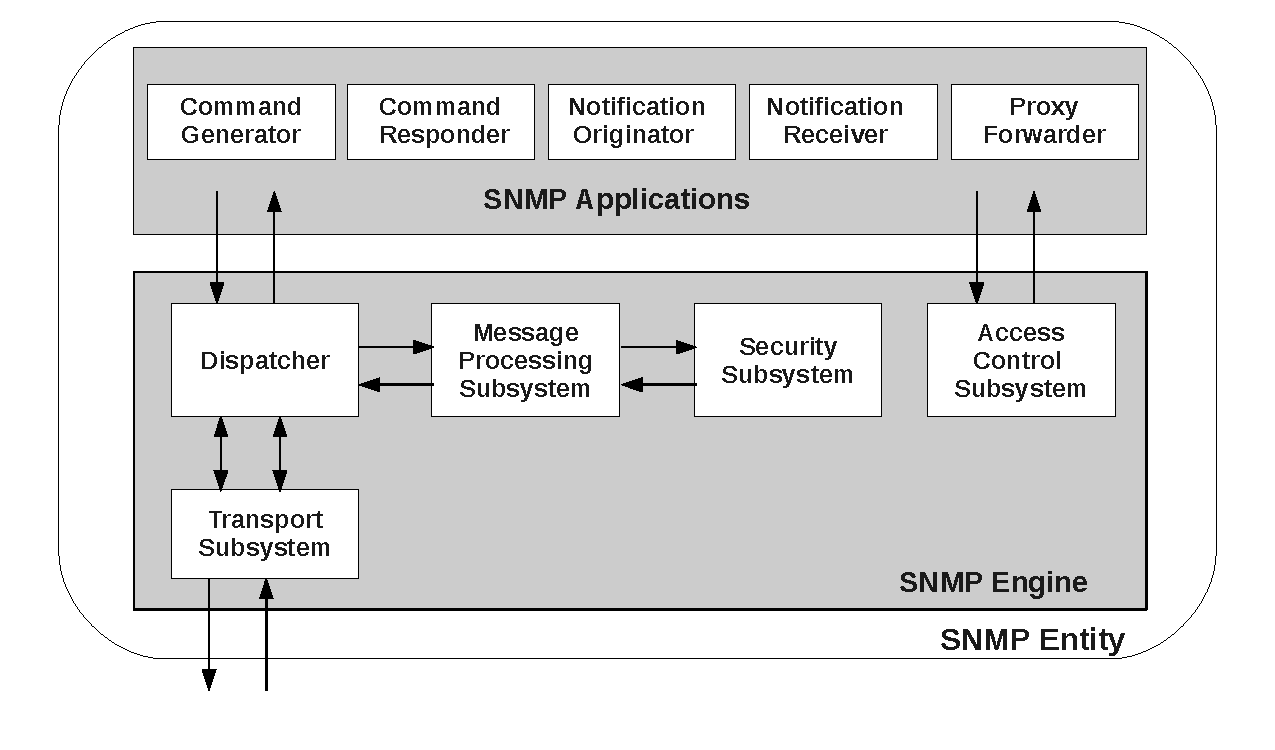
\includegraphics[scale = 0.6]{img/snmp-arch.pdf}
    \caption{Structure of an SNMP entity}   
	\label{fig:snmparch}
\end{center}
\end{figure}

According to the SNMP architecture defined in \cite{rfc3411}, an SNMP entity consists of an SNMP engine and one or more associated applications. The SNMP engine contains  a dispatcher, a message processing subsystem, a security subsystem, an access control subsystem, and a transport subsystem (Figure \ref{fig:snmparch}). Each subsystem may include multiple concrete models implementing different services. The dispatcher is responsible for controlling the data flow within an SNMP entity. Extracting data from received messages and preparing messages for sending are accomplished in the message processing subsystem. Each message processing model defines the format of a particular version of an SNMP message. Typically, the message processing subsystem supports three models for SNMPv1, SNMPv2c, and SNMPv3. The security subsystem provides security services such as authentication and privacy of messages. Authorization services are provided by the access control subsystem. The transport subsystem \cite{rfc5590} allows for multiple transport protocols to be used.

There are several types of defined applications (Figure \ref{fig:snmparch}), such as a command generator which monitor and manipulate management data, a command responder providing access to management data, a notification originator initiating asynchronous messages, a notification receiver processing these messages, and a proxy forwarder which forwards messages between entities. Applications may use the services provided by the SNMP engine. An SNMP entity which includes one or more command generator and notification receiver applications is called an SNMP manager. An entity containing one or more command generator and notification receiver applications is called an SNMP manager.


\section{Operations}

\section{Security Models}

 %%
%%
%   Conclusion
%%
\chapter{Proposed work}\label{ch:proposal}

The proposed Master Thesis is aimed at investigating whether the SNMP protocol may be reused "as is" in 802.15.4 networks. For this purpose, its implementation and evaluation for devices supporting IEEE 802.15.4 and running the Contiki Embedded Operating System \cite{contiki} will be accomplished. The target hardware platform will be the AVR Raven board which has a 2.4 GHz transceiver and uses an 8-bit ATmega1284P micro-controller with 16KB of RAM and 128KB of flash memory. The implementation will be done on top of the Contiki 6LoWPAN implementation.

The work will be accomplished over several phases. In the first phase, the basic SNMPv1 protocol will be implemented. Then, the focus will be shifted to the creation of a secure network layer for Contiki. Finally, a security layer will be added to the SNMPv1 implementation.

%Network Management: One of the points of transmitting IPv6
%       packets is to reuse existing protocols as much as possible.
%       Network management functionality is critical for LoWPANs.
%       However, management solutions need to meet the resource
%       constraints as well as the minimal configuration and self-healing
%       functionality described in Section 4.4. The Simple Network
%       Management Protocol (SNMP) [RFC3410] is widely used for
%       monitoring data sources and sensors in conventional networks.
%       SNMP functionality may be translated "as is" to LoWPANs with the
%       benefit to utilize existing tools.  However, due to the memory,
%       processing, and message size constraints, further investigation
%       is required to determine if the use of SNMPv3 is suitable, or if
%       an appropriate adaptation of SNMPv3 or use of different protocols
%       is in order.


% Bibliography
\newpage
\bibliographystyle{plain}
\bibliography{msc-proposal}
\addcontentsline{toc}{chapter}{Bibliography}

\nocite{ieee802.15.4}
\nocite{eui64}
\nocite{rfc780}
\nocite{rfc2460}
\nocite{rfc2464}
\nocite{rfc2474}
\nocite{rfc3168}
\nocite{rfc3775}
\nocite{rfc4191}
\nocite{rfc4291}
\nocite{rfc4443}
\nocite{rfc4861}
\nocite{rfc4862}
\nocite{rfc4919}
\nocite{rfc4944}
\nocite{draft-usecases-05}
\nocite{draft-hc-06}
\nocite{draft-nd-07}
\nocite{draft-routing-04}
\nocite{draft-protocols-07}
\nocite{draft-rpl-04}
\nocite{draft-routing-metrics-04}
\nocite{rfc1157}
\nocite{rfc1901}
\nocite{rfc1908}
\nocite{rfc3411}
\nocite{rfc3418}
\end{document}
